% =====================================================================
%  The same answer, two ways — brute-force spin-up vs. the flux-anchored
%  equilibrium solver. A focused argument (math + measurement) that the
%  old and new methods reach the same periodic steady state.
%  Self-contained for Overleaf: upload this folder (equivalence.tex +
%  figures/).  Compile: latexmk -pdf equivalence.tex
% =====================================================================
\documentclass[11pt]{article}

\usepackage[a4paper,margin=2.3cm]{geometry}
\setlength{\emergencystretch}{3em}
\usepackage[T1]{fontenc}
\usepackage{lmodern}
\usepackage{microtype}
\usepackage{amsmath,amssymb}
\usepackage{graphicx}
\usepackage{booktabs}
\usepackage{xcolor}
\usepackage[most]{tcolorbox}
\usepackage{enumitem}
\usepackage{titlesec}
\usepackage[hidelinks]{hyperref}

% ---- palette (matches the figures) ----
\definecolor{forest}{HTML}{3D6E4A}
\definecolor{coral}{HTML}{B85B3A}
\definecolor{char}{HTML}{2B2B2B}
\definecolor{dim}{HTML}{6B6B6B}
\definecolor{rulec}{HTML}{D8D2C8}
\hypersetup{colorlinks=true,allcolors=forest}

\titleformat{\section}{\normalfont\sffamily\large\bfseries\color{forest}}{\thesection}{0.6em}{}
\titleformat{\subsection}{\normalfont\sffamily\bfseries\color{char}}{\thesubsection}{0.5em}{}
\newcommand{\code}[1]{{\ttfamily\small #1}}
\newcommand{\Tm}{\langle T\rangle}

\newtcolorbox{plain}[1][]{colback=forest!6,colframe=forest!55,boxrule=0.6pt,
  arc=2pt,left=8pt,right=8pt,top=5pt,bottom=5pt,
  title={\sffamily\bfseries In plain words},coltitle=forest,fonttitle=\small,#1}
\newtcolorbox{key}[1][]{colback=coral!7,colframe=coral!60,boxrule=0.8pt,
  arc=2pt,left=8pt,right=8pt,top=5pt,bottom=5pt,
  title={\sffamily\bfseries The crux},coltitle=coral,fonttitle=\small,#1}
\newtcolorbox{meas}[1][]{colback=black!4,colframe=dim,boxrule=0.6pt,
  arc=2pt,left=8pt,right=8pt,top=5pt,bottom=5pt,
  title={\sffamily\bfseries What we measured},coltitle=char,fonttitle=\small,#1}

\begin{document}

\begin{center}
{\sffamily\bfseries\LARGE\color{forest} The same answer, two ways\par}
\vspace{2mm}
{\sffamily\large Brute-force spin-up vs.\ the flux-anchored equilibrium solver\par}
\vspace{2mm}
{\color{dim} Why the old and new methods must reach the same periodic steady
state --- the argument, and the measurement.\\
R.\,P.\ Gregorio \textperiodcentered\ Kasai Laboratory, Institute of Science Tokyo}
\end{center}
\vspace{2mm}
\hrule
\vspace{4mm}

\noindent
\textbf{Claim.} The fast flux-anchored solver (\code{lunar/equilibrium.py})
and a long brute-force spin-up are not two different models. They are two
\emph{routes to the same fixed point}: the unique periodic steady state of
the regolith column. This note proves that --- first by argument (the steady
state is unique and both methods land on it), then by measurement (brute
force, started from two very different temperatures, converges onto the
shortcut's profile).

% =====================================================================
\section{What ``the answer'' actually is}
% =====================================================================

Both methods solve the same 1-D heat equation in the regolith,
\begin{equation}
\rho(z)\,c_p(T)\,\frac{\partial T}{\partial t}
   = \frac{\partial}{\partial z}\!\left(K(T,z)\,\frac{\partial T}{\partial z}\right),
\label{eq:heat}
\end{equation}
with the same boundary conditions: a non-linear radiative balance at the
surface, and a fixed geothermal flux $Q_b$ entering at the bottom. Driven by
a periodic Sun, the column settles to a \emph{periodic steady state} ---
a temperature field $T(z,t)$ that repeats every lunation. That settled state
is ``the answer'' we want; the retrieval then asks which $K_d$ makes it match
the sensors.

The periodic steady state is pinned by two conditions:

\begin{enumerate}[leftmargin=1.6em,itemsep=2pt]
\item \textbf{The surface skin is periodic.} In the top few skin depths the
temperature swings through a repeating daily cycle set by the radiative
balance.
\item \textbf{The deep column carries exactly $Q_b$.} Below the skin there
are no heat sources, so in steady state the cycle-mean conductive flux is the
\emph{same at every depth} --- and that value is the flux entering from below,
$Q_b$. Writing the cycle mean as $\Tm$,
\begin{equation}
K\bigl(\Tm,z\bigr)\,\frac{d\Tm}{dz} \;=\; Q_b
\qquad\Longrightarrow\qquad
\frac{d\Tm}{dz} \;=\; \frac{Q_b}{K(\Tm,z)} .
\label{eq:flux}
\end{equation}
\end{enumerate}

\begin{plain}
Condition~2 is just conservation of energy at steady state: with nothing
adding or removing heat inside the rock, the same trickle of geothermal heat
($Q_b$) must pass through every layer. That \emph{fixes how fast temperature
rises with depth} --- the gradient is $Q_b$ divided by the conductivity. The
deep temperature profile is therefore \emph{not a free thing to be
discovered}; it is determined by Eq.~\eqref{eq:flux} once you know the
temperature at any one depth.
\end{plain}

% =====================================================================
\section{The old way: brute-force spin-up}
% =====================================================================

Start the column at some guessed temperature and integrate
Eq.~\eqref{eq:heat} forward, lunation after lunation, until it stops
changing. This is correct in the limit of infinite time --- but the catch is
\emph{how long} that takes. The column relaxes on the diffusive timescale of
its full depth,
\begin{equation}
\tau \sim \frac{z_{\max}^2}{\kappa}
\;\approx\; \text{order } 10^{3}\ \text{lunations}
\qquad (z_{\max}=5\,\text{m},\ \kappa\sim10^{-8}\,\text{m}^2\text{s}^{-1}).
\end{equation}
A fixed spin-up of a few tens of lunations is nowhere near that. At the
sensor depths (0.8--2.4\,m) the profile still \emph{remembers the temperature
it was started at}.

\begin{tcolorbox}[colback=coral!6,colframe=coral!55,boxrule=0.6pt,arc=2pt,
  title={\sffamily\bfseries The old trap (audit flag F1)},coltitle=coral,fonttitle=\small]
Because the deep relaxation is so slow, the usual convergence check ---
``did $\Tm$ change by less than $0.01$\,K between successive lunations?'' ---
\emph{passes long before the column is actually settled}. The model looks
converged while it is still drifting. The starting temperature then acts as a
hidden free parameter, and it biases the retrieved $K_d$. That is the bug the
new method removes: not by running longer, but by not needing to.
\end{tcolorbox}

% =====================================================================
\section{The new way: the flux-anchored shortcut}
% =====================================================================

The shortcut does not wait for diffusion to \emph{discover}
Eq.~\eqref{eq:flux} --- it \emph{imposes} it. One outer iteration is:

\begin{enumerate}[leftmargin=1.6em,itemsep=3pt]
\item \textbf{Short spin-up ($\sim$12 lunations).} Long enough to make the
fast surface skin periodic against the current deep column, and to read the
cycle-mean ``anchor'' temperature $\Tm(z_0)$ just below the skin
($z_0\approx0.55$\,m). The skin is fast because its relaxation time is small,
and its mean temperature is set by the surface balance --- which barely cares
about the deep column ($Q_b$ is $\sim10^{-4}$ of the diurnal flux scale).
\item \textbf{Reconstruct the deep profile.} From the anchor, integrate
Eq.~\eqref{eq:flux} downward to fill in $\Tm(z)$ for all $z>z_0$ ---
\emph{instantly}, no time-stepping. (A small ``rectified'' eddy term
$u_{\rm rect}=\langle K\,\partial_zT\rangle-K(\Tm)\,\partial_z\Tm$ is computed
from the cycle and subtracted, so the closure stays exact near the skin.)
\item \textbf{Iterate.} Feed the reconstructed column back into another short
spin-up and repeat. It converges in 3--5 rounds.
\end{enumerate}

\begin{plain}
Same destination, no waiting. Like finding a tank's steady water level from
``inflow $=$ outflow'' instead of pouring water in and watching it slosh for
an hour. The level is fixed by a balance; you can compute it directly.
\end{plain}

% =====================================================================
\section{Why they cannot disagree}
% =====================================================================

This is the part worth being precise about.

\begin{enumerate}[leftmargin=1.6em,itemsep=3pt]
\item \textbf{The steady state is unique.} Given the anchor value
$\Tm(z_0)$, Eq.~\eqref{eq:flux} is a first-order ODE with a smooth
right-hand side, so it has \emph{one} solution below the anchor. The anchor
value itself is set by the surface energy balance, which the skin reaches
quickly and essentially independently of the deep column. So there is exactly
one periodic steady state.
\item \textbf{Brute force reaches it.} Equation~\eqref{eq:heat} is a
parabolic equation with periodic forcing. Its transient decays on the
timescale $\tau$, and what remains is the unique periodic response. So
brute-force-to-convergence \emph{is} that unique state --- it just spends
$\sim10^3$ lunations getting there.
\item \textbf{The shortcut reaches it.} Its fixed point satisfies condition~1
(the skin is periodic, by step~1) \emph{and} condition~2 (flux closure, by
step~2) --- the two conditions that define the steady state. So its fixed
point is the same unique state.
\end{enumerate}

\begin{key}
The two methods enforce the \emph{same} two conditions; the steady state
satisfying them is \emph{unique}. The only difference is bookkeeping: brute
force discovers the deep gradient $Q_b/K$ slowly, by letting heat diffuse;
the shortcut writes it down directly from energy conservation. A different
final answer would require a second steady state --- and for this problem
there isn't one. \emph{They must agree.}
\end{key}

\noindent
The one honest caveat: the reconstruction uses the mean-field form of
Eq.~\eqref{eq:flux} plus the rectification correction, so the shortcut equals
the true steady state to a small, \emph{controlled} tolerance (tens of mK at
sensor depth, see below), not bit-for-bit. Brute force, in turn, only reaches
that same tolerance after thousands of lunations. So ``equal'' means ``equal
to within a tolerance both methods can be pushed below,'' which is exactly
what the measurement shows.

% =====================================================================
\section{The proof: they land on the same profile}
% =====================================================================

\paragraph{Convergence from a wrong start.} Starting brute force at
240\,K (the shortcut's settled value at 1\,m is 250.38\,K) and continuing,
the gap closes monotonically and exponentially:

\begin{center}\small
\begin{tabular}{@{}rccc@{}}
\toprule
brute-force lunations & $\Tm$ at 1\,m [K] & error vs.\ shortcut [K] \\
\midrule
100  & 244.48 & 5.90 \\
300  & 246.55 & 3.83 \\
600  & 248.19 & 2.19 \\
1000 & 249.36 & 1.02 \\
\midrule
\textbf{shortcut} & \textbf{250.38} & \textbf{(reference)} \\
\bottomrule
\end{tabular}
\end{center}

\noindent
The error roughly halves every few hundred lunations ($e$-folding
$\sim$520 lunations) --- a single exponential decaying onto the shortcut's
value. Extrapolated, brute force matches the shortcut's certified tolerance
at $\sim$3000 lunations.

\paragraph{Two starts, one curve.} Run brute force all the way (3000
lunations) from \emph{two} very different starts, 240\,K and 260\,K, and
overlay both on the shortcut (Figure~\ref{fig:demo}). The three profiles are
indistinguishable across the whole 5\,m column.

\begin{figure}[h]
\centering
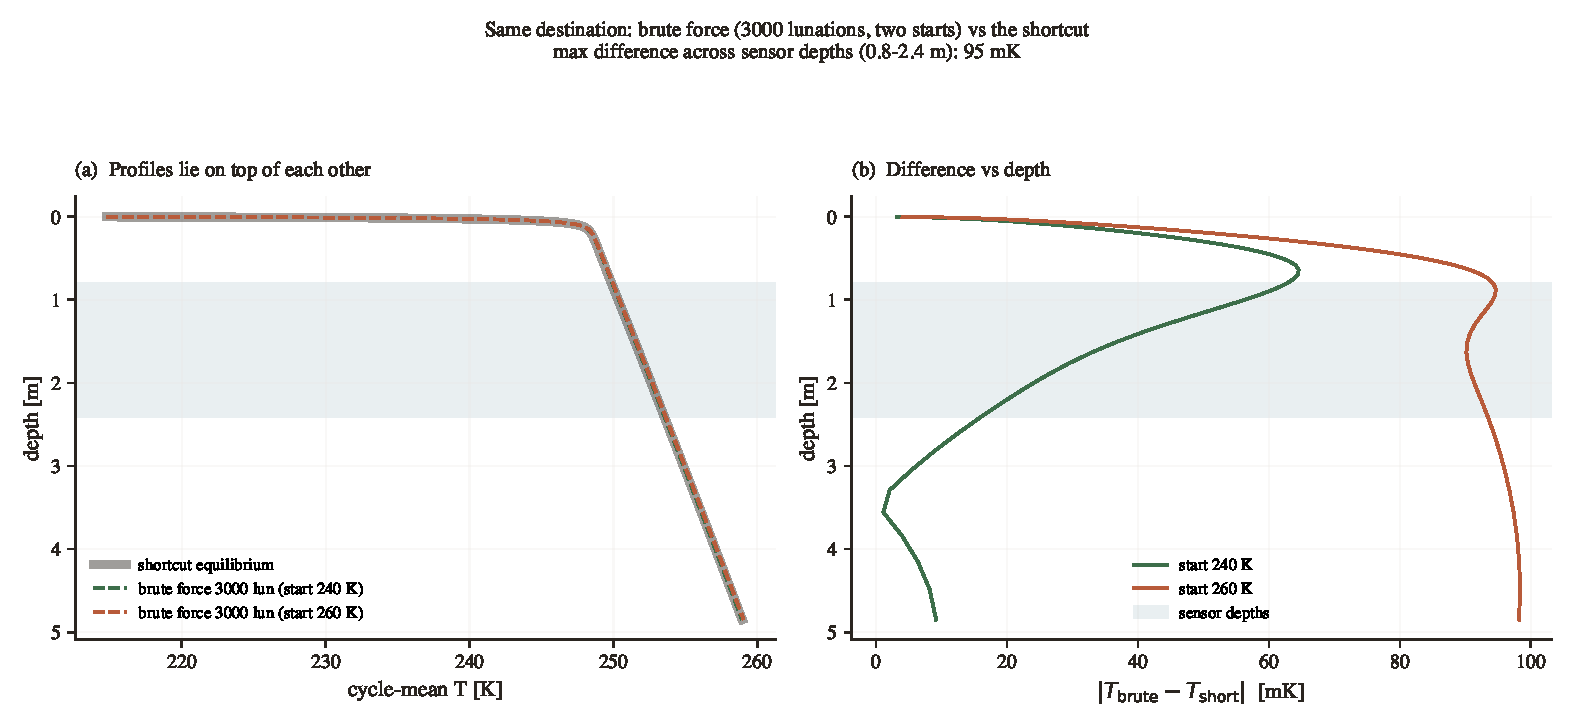
\includegraphics[width=\linewidth]{figures/fig_equilibrium_demo.pdf}
\caption{Brute force run to 3000 lunations from 240\,K \emph{and} 260\,K
(dashed), overlaid on the flux-anchored shortcut (solid grey). Left: the
profiles lie on top of one another. Right: the residual is at most
$\sim$60--95\,mK across the sensor depths --- and that remainder is simply
brute force still finishing the last fraction of its slow descent (it keeps
shrinking with more lunations). Two unrelated starting points and the direct
method all reach one profile.}
\label{fig:demo}
\end{figure}

\begin{meas}
\textbf{Quantitatively.} At 3000 lunations the fully-converged brute force
agrees with the shortcut to \textbf{63\,mK} (start 240\,K) and \textbf{95\,mK}
(start 260\,K) across the sensor depths (0.8--2.4\,m) --- and that gap is
still closing. The shortcut reaches the same state in $\sim$9\,s; brute force
needs $\sim$4\,min to match it.
\end{meas}

\paragraph{The shortcut certifies its own convergence.} It does not ask you
to trust it. Every solve returns two diagnostics
(Figure~\ref{fig:cert}): the anchor \emph{drift} between outer iterations
(required $<0.03$\,K; typically $\sim$3\,mK) and the \emph{flux closure},
$\max|\langle q\rangle-Q_b|/Q_b$ below the anchor (required $<2\%$). A direct
guess-independence test --- start the shortcut from 240\,K and 260\,K --- gives
sensor-depth temperatures agreeing to $<0.03$\,K. So the shortcut is provably
at the steady state, which is precisely the check the old fixed-spin-up could
not pass.

\begin{figure}[h]
\centering
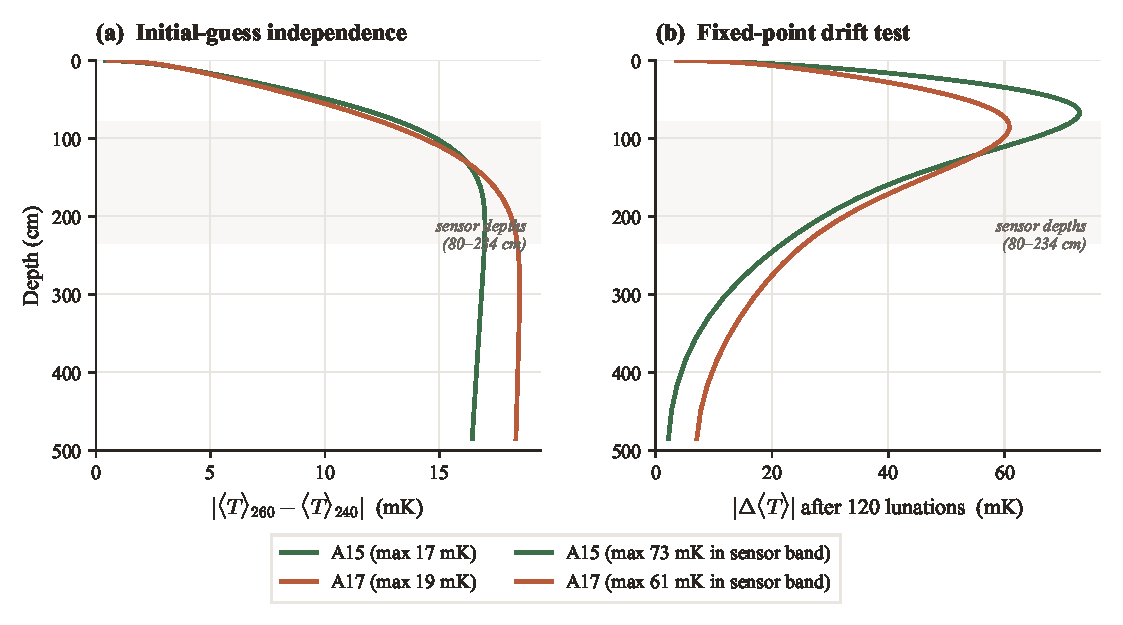
\includegraphics[width=0.82\linewidth]{figures/fig_equilibrium_certification.pdf}
\caption{Solver certification: guess-independence and mean-flux closure on
$Q_b$ as functions of depth/iteration. These are the numbers that \emph{prove}
the shortcut arrived at the periodic steady state.}
\label{fig:cert}
\end{figure}

% =====================================================================
\section{Bottom line}
% =====================================================================

\begin{itemize}[leftmargin=1.4em,itemsep=2pt]
\item \textbf{Same answer.} Both methods target the one periodic steady state.
Brute force from any start converges onto the shortcut's profile
(Figure~\ref{fig:demo}); the argument in \S4 says it has no choice.
\item \textbf{$\sim$30$\times$ less work.} The shortcut reaches it in
$\sim$9\,s; brute force needs $\sim$3000 lunations ($\sim$4\,min) per solve to
match --- and the retrieval needs hundreds of solves.
\item \textbf{And it is certified.} \code{drift} and \code{flux\_closure}
prove convergence on every solve, removing the hidden-parameter bias (F1)
that the old fixed-length spin-up silently carried.
\end{itemize}

\noindent
\textit{Reproduce it yourself:} \code{notebooks/equilibrium\_demo.ipynb} runs
both methods (the brute-force runs fan across CPU cores) and regenerates
Figure~\ref{fig:demo}; \code{pytest tests/test\_equilibrium.py} runs the
guess-independence and flux-closure checks.

\end{document}
